\newpage
\section{Aufgabe3}
\label{sec:a3}

\FloatBarrier
\begin{figure}
  \centering
  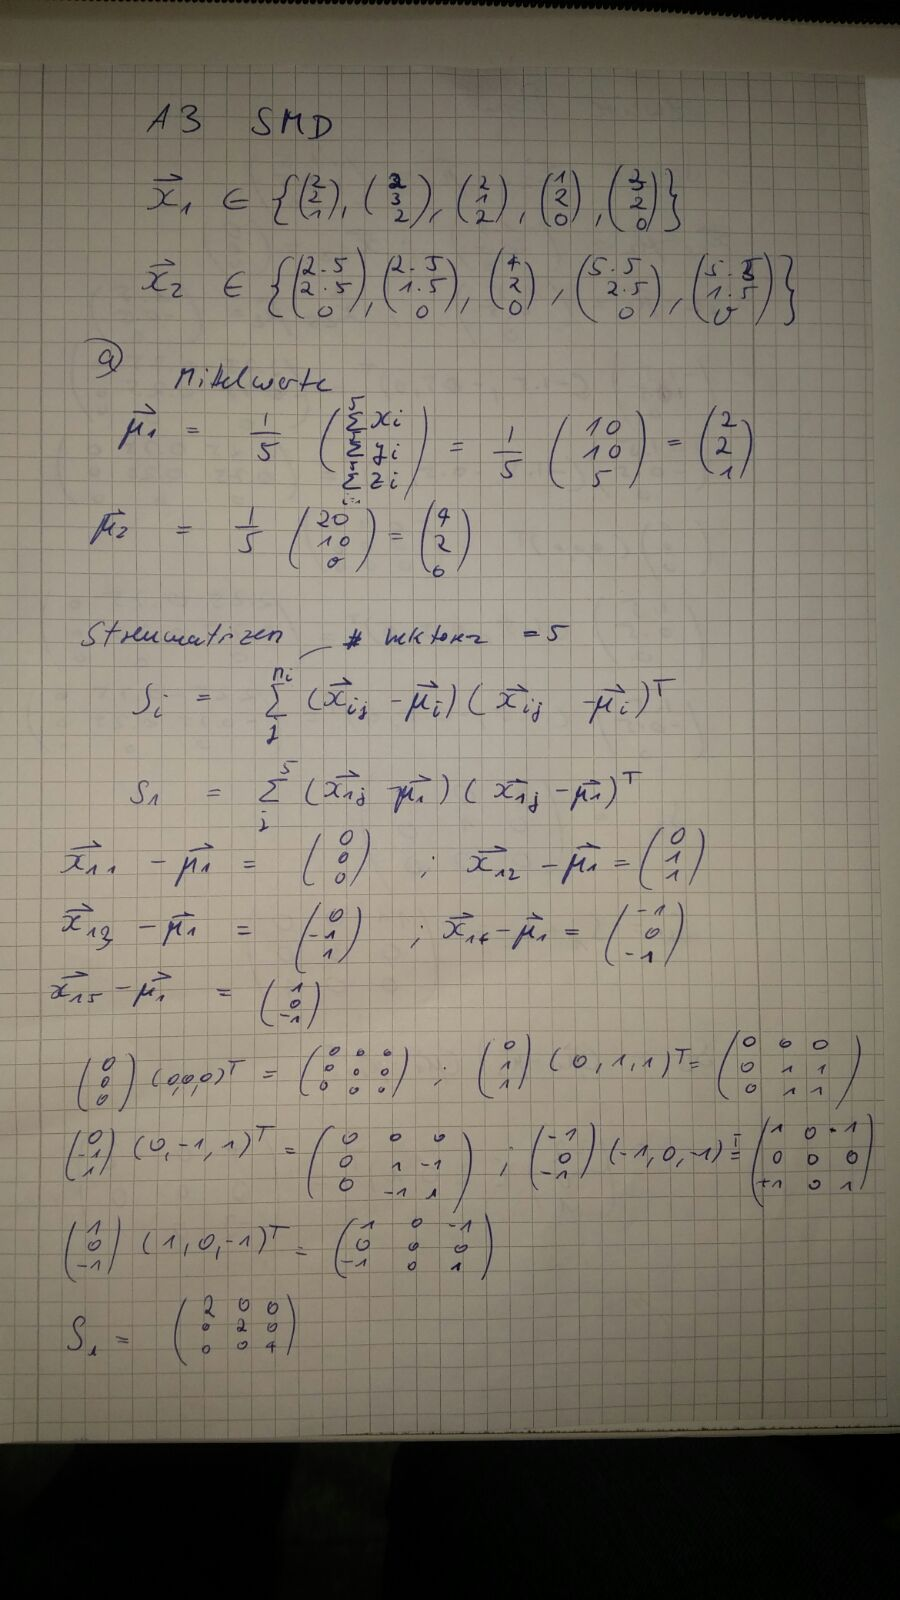
\includegraphics[width=\textwidth]{bild1.jpeg}
  \caption{}.
  \label{fig:1}
\end{figure}
\FloatBarrier

\FloatBarrier
\begin{figure}
  \centering
  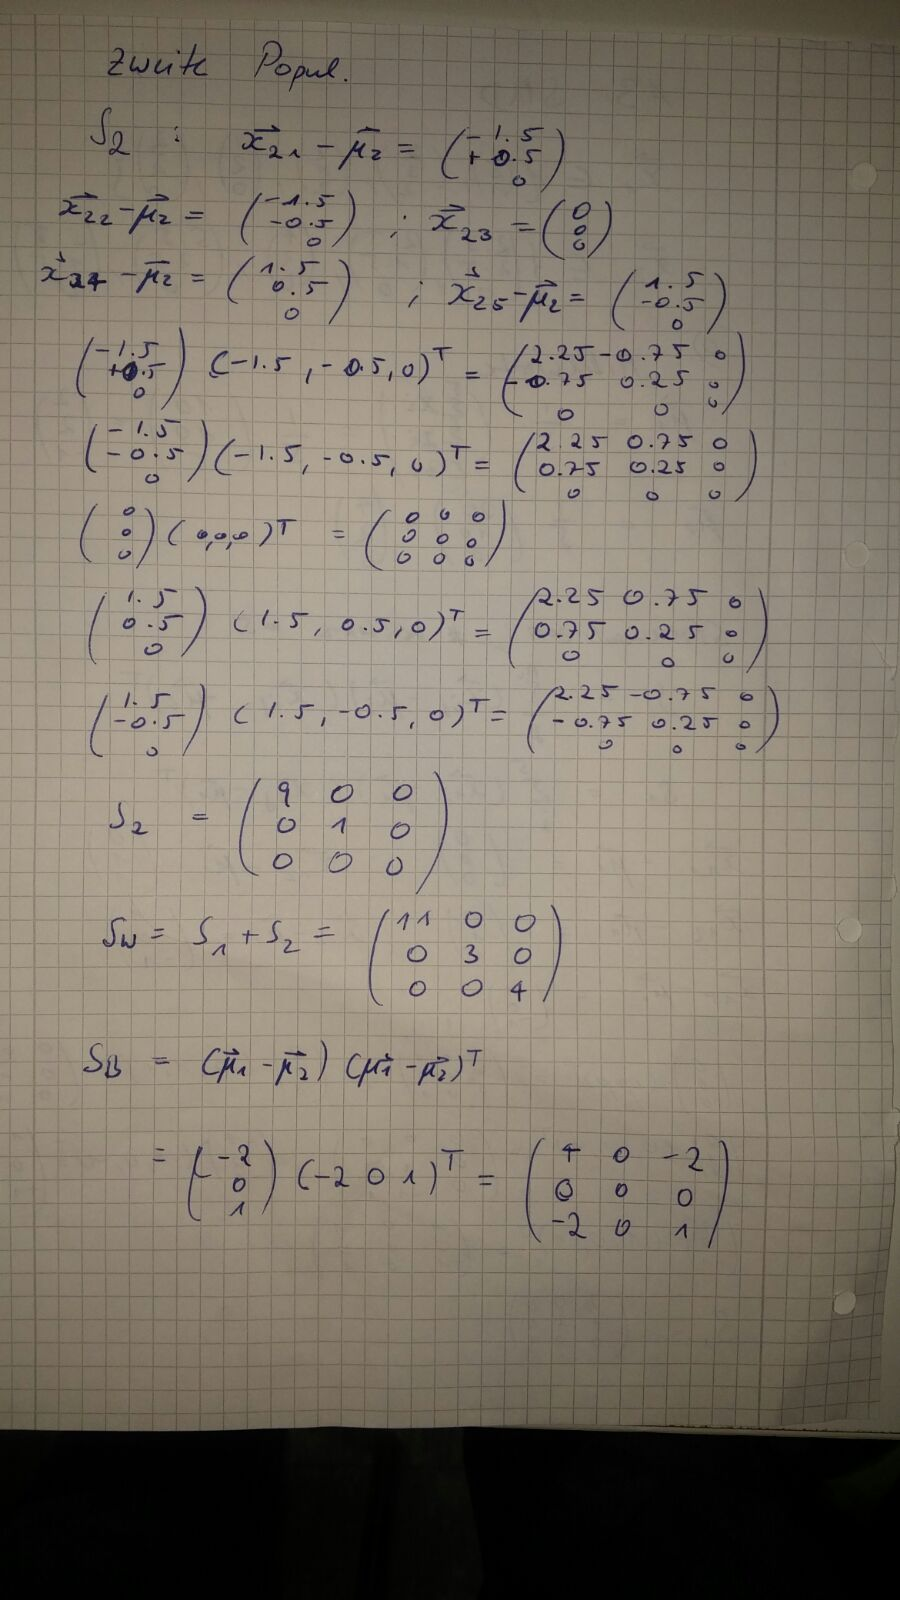
\includegraphics[width=\textwidth]{bild2.jpeg}
  \caption{}.
  \label{fig:2}
\end{figure}
\FloatBarrier

\FloatBarrier
\begin{figure}
  \centering
  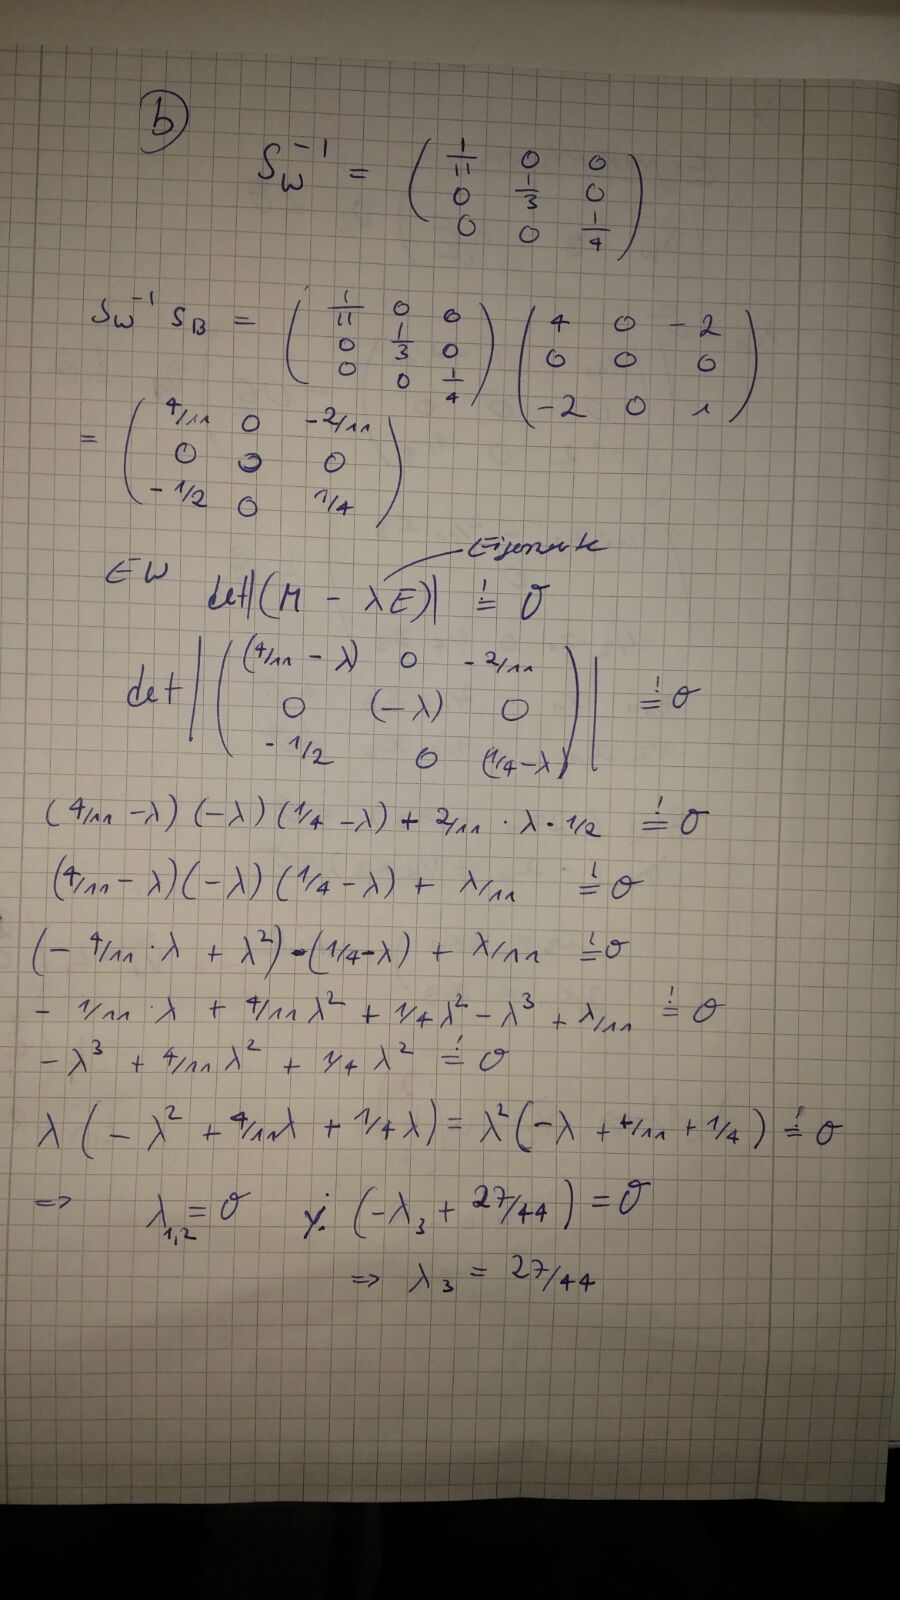
\includegraphics[width=\textwidth]{bild3.jpeg}
  \caption{}.
  \label{fig:3}
\end{figure}
\FloatBarrier

\FloatBarrier
\begin{figure}
  \centering
  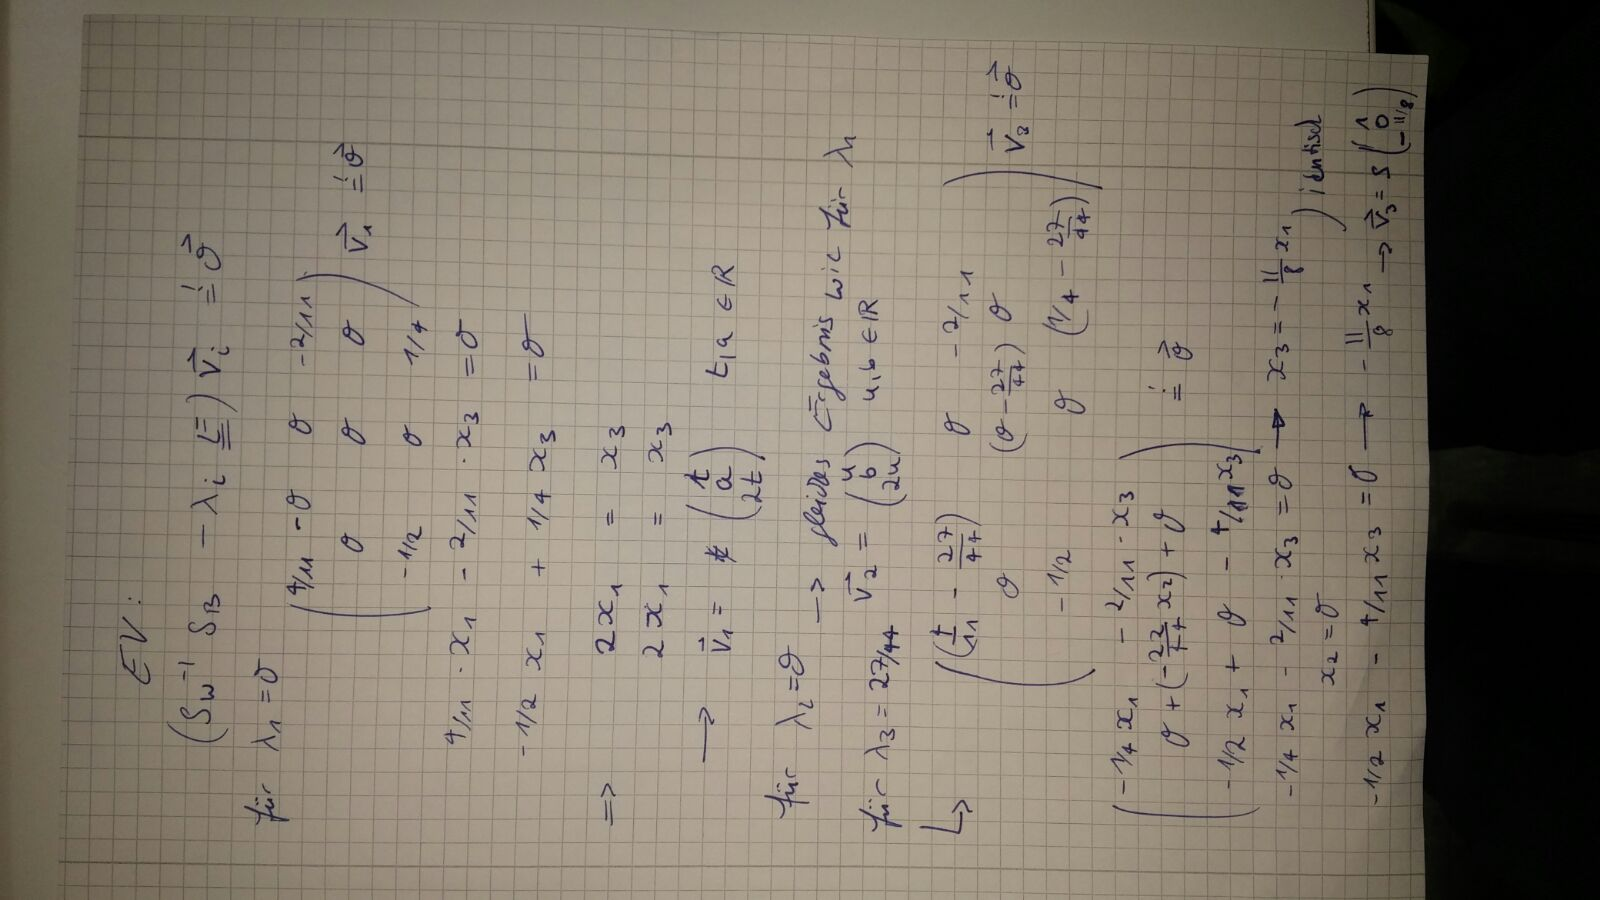
\includegraphics[width=\textwidth]{bild4.jpeg}
  \caption{}.
  \label{fig:4}
\end{figure}
\FloatBarrier

\FloatBarrier
\begin{figure}
  \centering
  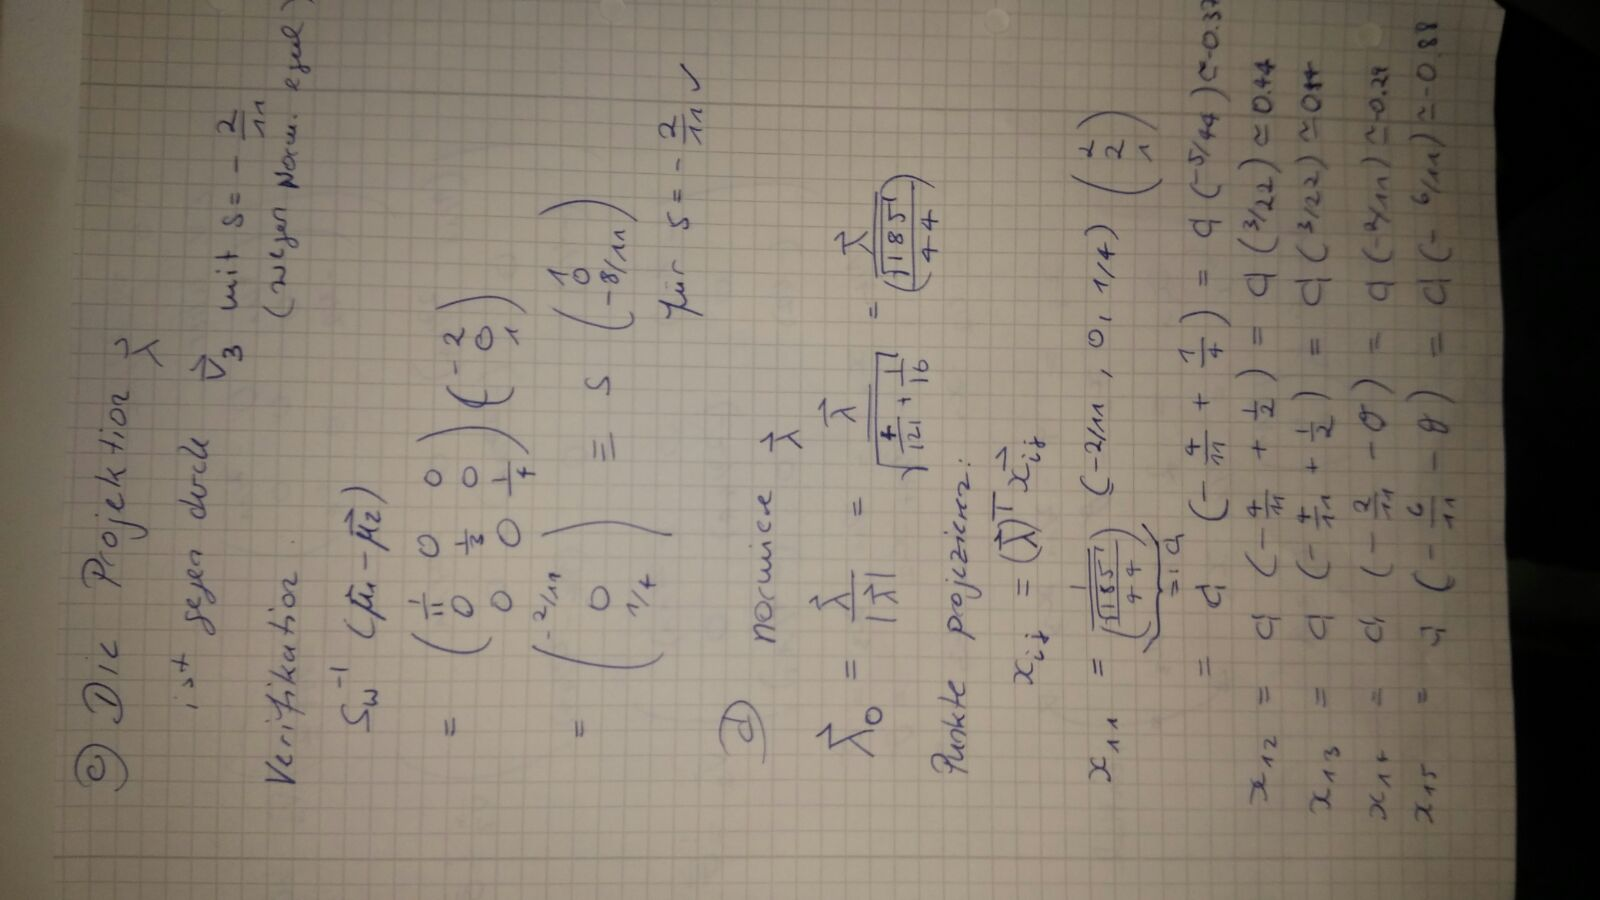
\includegraphics[width=\textwidth]{bild5.jpeg}
  \caption{}.
  \label{fig:5}
\end{figure}
\FloatBarrier

\FloatBarrier
\begin{figure}
  \centering
  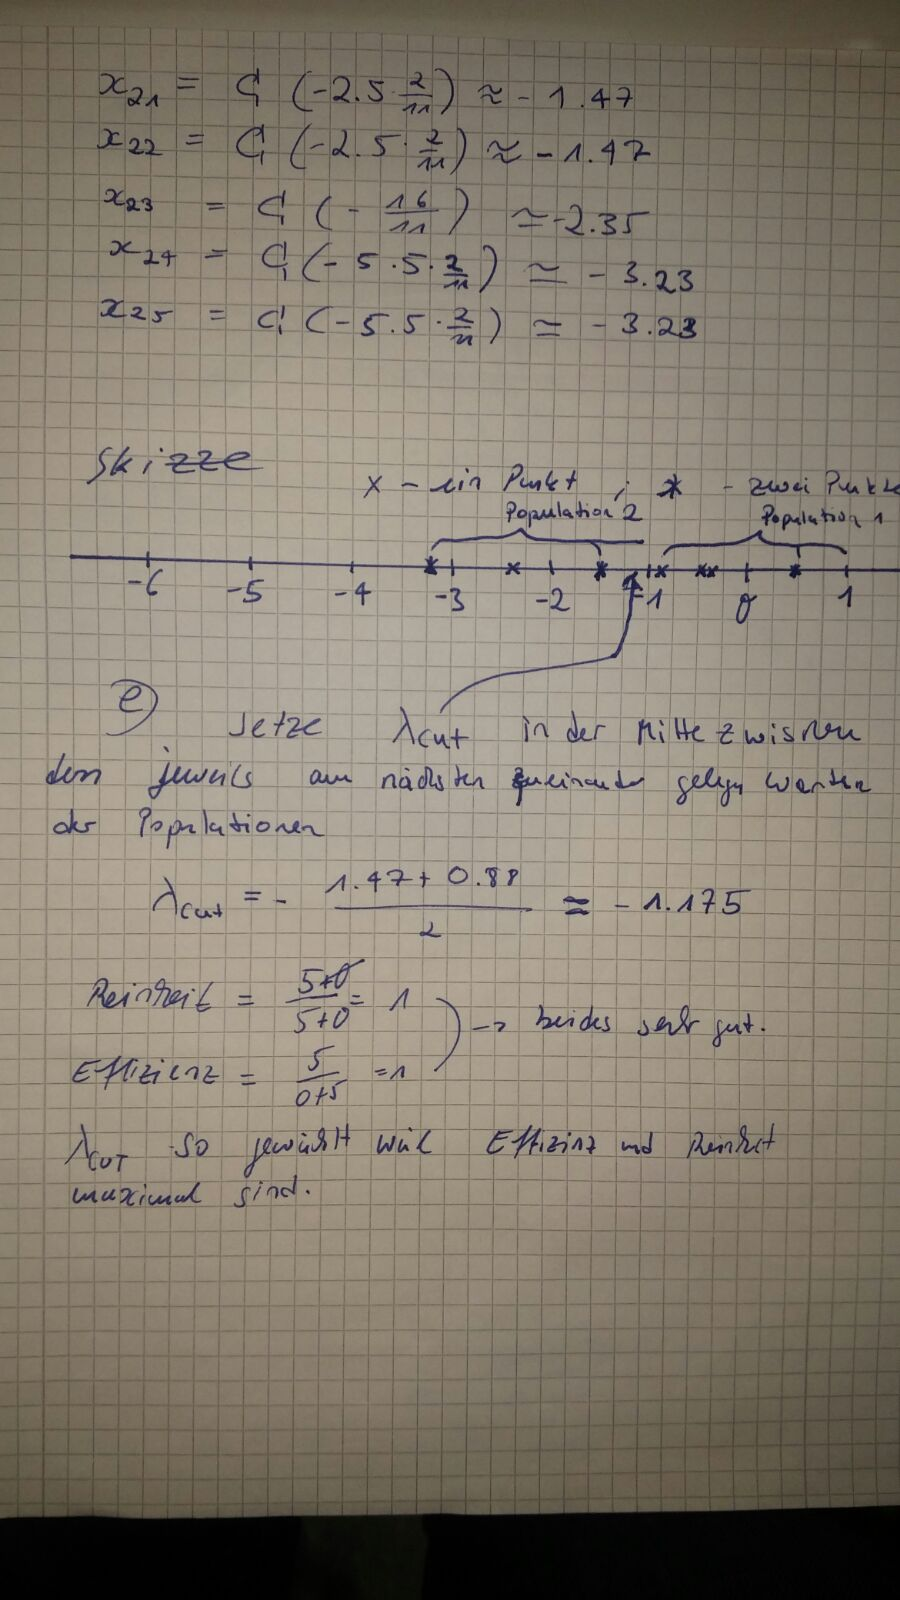
\includegraphics[width=\textwidth]{bild6.jpeg}
  \caption{}.
  \label{fig:6}
\end{figure}
\FloatBarrier
